\documentclass{ieeeaccess}
\usepackage{cite}
\usepackage{amsmath,amssymb,amsfonts}
\usepackage{graphicx}
\usepackage{textcomp}
\usepackage{hyperref}
\usepackage{booktabs}

\makeatletter
\AtBeginDocument{\DeclareMathVersion{bold}
\SetSymbolFont{operators}{bold}{T1}{times}{b}{n}
\SetSymbolFont{NewLetters}{bold}{T1}{times}{b}{it}
\SetMathAlphabet{\mathrm}{bold}{T1}{times}{b}{n}
\SetMathAlphabet{\mathit}{bold}{T1}{times}{b}{it}
\SetMathAlphabet{\mathbf}{bold}{T1}{times}{b}{n}
\SetMathAlphabet{\mathtt}{bold}{OT1}{pcr}{b}{n}
\SetSymbolFont{symbols}{bold}{OMS}{cmsy}{b}{n}
\renewcommand\boldmath{\@nomath\boldmath\mathversion{bold}}}
\makeatother

\def\BibTeX{{\rm B\kern-.05em{\sc i\kern-.025em b}\kern-.08em
    T\kern-.1667em\lower.7ex\hbox{E}\kern-.125emX}}

\begin{document}
\history{Date of version 25/05/2026}
\doi{}

\title{Statistical and Dimensionality-Reduction Analysis of the Communities and Crime Dataset}
\author{Serkan Eren\authorrefmark{1}}

\address[1]{Artificial Intelligence Graduate Program, Department of Computer Engineering, Faculty of Engineering, Gebze Technical University, Kocaeli, T\"urkiye}

\tfootnote{This work was conducted as the final project of the CSE 555: Statistical Pattern Recognition course in the Master's Degree Program at Gebze Technical University.}

\markboth
{S.~Eren: Statistical and Dimensionality-Reduction Analysis of the Communities and Crime Dataset}
{S.~Eren: Statistical and Dimensionality-Reduction Analysis of the Communities and Crime Dataset}

\corresp{s.eren2018@gtu.edu.tr}

\begin{abstract}
This work investigates the structure of the UCI \emph{Communities and Crime} dataset through a sequence of exploratory, statistical, and dimensionality-reduction analyses. A curated subset of eighteen normalized sociodemographic variables is studied together with a three-level discretization of the continuous target \texttt{ViolentCrimesPerPop} into Low, Medium, and High crime classes by tertiles. The pipeline includes per-feature box-plot inspection and Isolation-Forest-based multivariate outlier cleaning, Pearson and Spearman correlation analysis, z-score normalization with per-feature Fisher Distance, principal component analysis (PCA) with Fisher Distance per principal component, linear discriminant analysis (LDA), and a comparison of K-Means, DBSCAN, t-SNE, and Self-Organizing Map projections. Quantitative separability is reported through silhouette and 5-NN cross-validation accuracy on the 2-D embeddings, and the SOM organisation is summarised by a per-neuron class-purity hit-map. The analysis confirms that family-structure and socioeconomic variables (e.g., \texttt{PctKids2Par}, \texttt{PctIlleg}, \texttt{PctPopUnderPov}) carry the strongest individual class signal, that the leading PCA component inherits most of this discriminative content, and that LDA produces a tighter class-separable 2-D embedding than PCA. A Welch's t-test on \texttt{PctKids2Par} between Low and High classes confirms a highly significant mean difference at both $n=36$ and $n=64$.
\end{abstract}

\begin{keywords}
Communities and Crime, exploratory data analysis, Fisher Distance, PCA, LDA, K-Means, DBSCAN, t-SNE, Self-Organizing Map, hypothesis testing.
\end{keywords}

\titlepgskip=-21pt
\maketitle

% ===================================================================
\section{Introduction}
\label{sec:introduction}
\PARstart{T}{he} \emph{Communities and Crime} dataset from the UCI Machine Learning Repository \cite{uciccrime} is a widely used benchmark for sociodemographic modelling of community-level violent crime in the United States. It aggregates information from the 1990 U.S.~Census, the 1990 U.S.~Law Enforcement Management and Administrative Statistics (LEMAS) survey, and the 1995 FBI Uniform Crime Reports (UCR), and contains $1\,994$ communities described by $128$ attributes. Each predictive attribute is already normalized to the $[0,1]$ interval by the dataset authors so that comparisons across communities of different population are meaningful.

The aim of this study is not to build a competitive predictive model, but to apply the statistical and pattern-recognition tools taught in CSE 555 to a real, mixed-quality dataset, and to interpret what each tool exposes about the data. To reduce dimensionality to a tractable yet representative working set, eighteen sociodemographic variables covering age structure, ethnic composition, education, employment, family stability, housing, and immigration are selected (Table~\ref{tab:features}). To obtain a multi-class problem as required by the assignment, the continuous response \texttt{ViolentCrimesPerPop} is discretized into three equal-frequency classes \emph{Low}, \emph{Medium}, and \emph{High} by its tertiles.

The remainder of the paper is organized as follows. Section~\ref{sec:dataset} describes the dataset and the preprocessing pipeline. Sections~\ref{sec:boxplot}--\ref{sec:hypothesis} address the eight analytical tasks of the project in order: distributions and outliers (Section~\ref{sec:boxplot}), correlation analysis (Section~\ref{sec:corr}), per-feature Fisher Distance after z-scoring (Section~\ref{sec:fisher}), PCA-based Fisher analysis (Section~\ref{sec:pca}), top/bottom PC scatter plots (Section~\ref{sec:pcscatter}), LDA (Section~\ref{sec:lda}), clustering with K-Means, DBSCAN, t-SNE, and SOM (Section~\ref{sec:cluster}), and a Welch t-test (Section~\ref{sec:hypothesis}). Section~\ref{sec:conclusion} summarizes the main findings.

% ===================================================================
\section{Dataset and Preprocessing}
\label{sec:dataset}
The Communities and Crime dataset \cite{uciccrime} contains $1\,994$ rows and $128$ columns, of which five are non-predictive identifiers (\texttt{state}, \texttt{county}, \texttt{community}, \texttt{communityname}, \texttt{fold}). A non-trivial fraction of the LEMAS-derived columns is missing for most communities; those columns were therefore excluded from the working subset. After identifier removal, a curated set of $18$ sociodemographic features (Table~\ref{tab:features}) was selected based on (i) low missingness, (ii) interpretability for crime-related analysis, and (iii) coverage of distinct conceptual domains (demographics, economy, education, family, housing, immigration). The continuous response \texttt{ViolentCrimesPerPop} was discretized by tertiles into three classes \emph{Low}, \emph{Medium}, and \emph{High} (679 / 662 / 653 samples before cleaning).

\begin{table}[!t]
\caption{Selected features and their interpretation. All values are normalized to $[0,1]$ by the dataset authors.}
\label{tab:features}
\centering
\small
\begin{tabular}{p{2.3cm}p{5.5cm}}
\toprule
Feature & Description \\
\midrule
\texttt{population} & Community population \\
\texttt{householdsize} & Mean household size \\
\texttt{racepctblack} & Percent of Black population \\
\texttt{racePctWhite} & Percent of White population \\
\texttt{agePct12t29} & Percent of population aged 12--29 \\
\texttt{agePct65up} & Percent of population aged $\geq 65$ \\
\texttt{pctUrban} & Percent of population living in urban areas \\
\texttt{medIncome} & Median household income \\
\texttt{PctPopUnderPov} & Percent of population under poverty line \\
\texttt{PctNotHSGrad} & Percent without a high-school diploma \\
\texttt{PctBSorMore} & Percent with a Bachelor's degree or higher \\
\texttt{PctUnemployed} & Percent unemployed \\
\texttt{MalePctDivorce} & Percent of divorced males \\
\texttt{PctKids2Par} & Percent of kids in two-parent households \\
\texttt{PctIlleg} & Percent of children born to never-married parents \\
\texttt{NumImmig} & Number of foreign-born residents \\
\texttt{PctHousOwnOcc} & Percent of owner-occupied housing units \\
\texttt{PctVacantBoarded} & Percent of boarded-up vacant housing \\
\bottomrule
\end{tabular}
\end{table}

Any residual missing values in the working subset were imputed by the per-column median. All subsequent analyses were carried out in Python~3.10 using \texttt{NumPy}, \texttt{pandas}, \texttt{scikit-learn}~\cite{pedregosa}, \texttt{scipy}, \texttt{seaborn}, and \texttt{MiniSom}~\cite{minisom}. The complete Jupyter notebook accompanies this report.

% ===================================================================
\section{Distributions and Outlier Detection (Task 1)}
\label{sec:boxplot}
Figure~\ref{fig:box_before} presents per-feature box plots of the eighteen selected variables before outlier removal. Several features are visibly right-skewed and exhibit a long upper tail of extreme values --- most notably \texttt{population}, \texttt{NumImmig}, \texttt{PctIlleg}, \texttt{PctVacantBoarded}, and \texttt{PctPopUnderPov}. These tails reflect a small set of communities that are demographically or socioeconomically extreme (very large cities, communities with very high immigration counts, or extreme deprivation). In contrast, variables such as \texttt{agePct12t29}, \texttt{agePct65up}, and \texttt{householdsize} are tightly concentrated around the population median with comparatively few outliers.

\begin{figure}[!t]
\centering
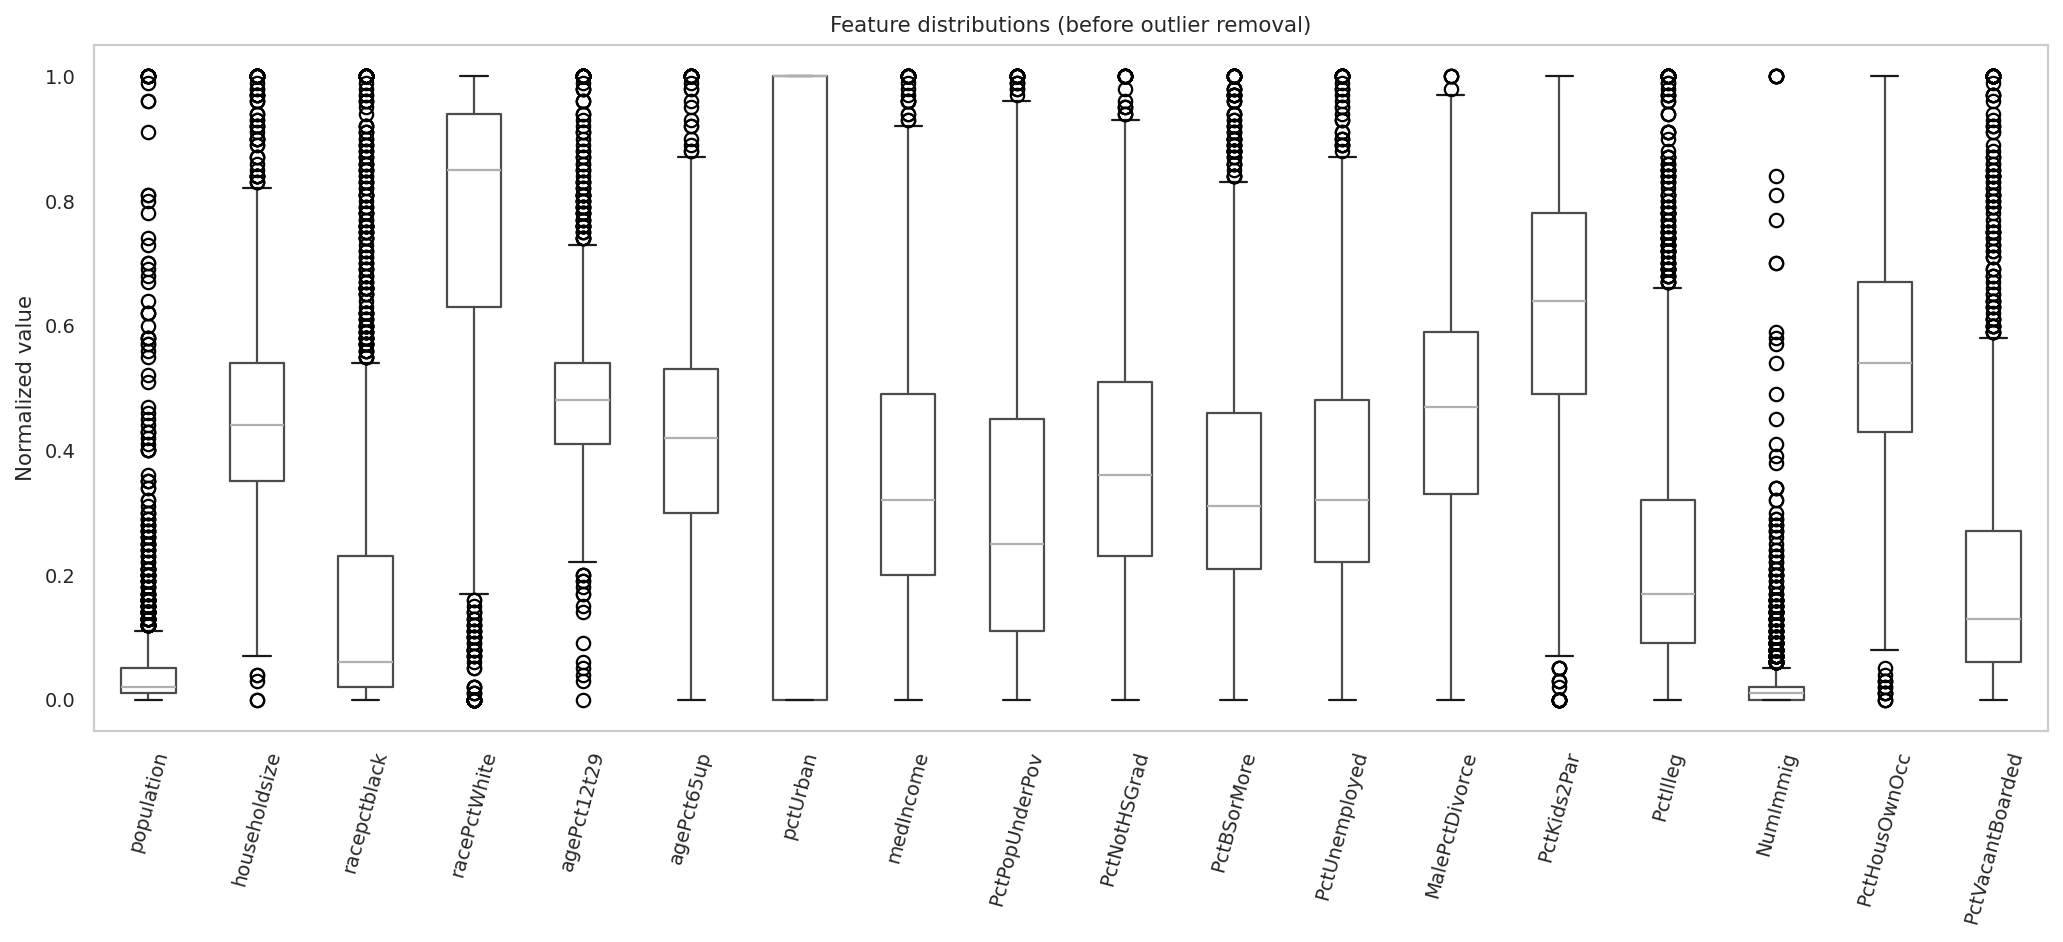
\includegraphics[width=\columnwidth]{boxplot_before.png}
\caption{Box plots of the eighteen selected features prior to outlier removal. Several socioeconomic variables show clear right-skew with long upper tails.}
\label{fig:box_before}
\end{figure}

A multivariate outlier detector was preferred over a per-feature filter (e.g.\ univariate IQR rejection), because the latter discards any sample that is extreme on \emph{any} dimension. In a sociodemographic dataset such as this one, several class-discriminative features (\texttt{PctPopUnderPov}, \texttt{PctIlleg}, \texttt{PctVacantBoarded}) intrinsically have heavy upper tails populated almost exclusively by High-crime communities, so a per-feature rule would severely deplete the High-crime class and bias every subsequent analysis. As a preliminary experiment, applying a per-feature IQR rule with multiplier $k=3$ removed $358$ rows ($18.0\%$) and shrank the High-crime class from $653$ to $418$ samples --- an imbalance large enough to distort the supervised analyses of Sections~\ref{sec:fisher}--\ref{sec:lda}.

The final pipeline therefore uses the multivariate \emph{Isolation Forest} \cite{liu2008isolation} of \texttt{scikit-learn} \cite{pedregosa} with $200$ trees and a contamination rate of $5\%$. The detector isolates each sample by recursive random partitioning of the feature space; samples that are isolated with unusually short paths are flagged as anomalous. With contamination $=0.05$ the filter removes $100$ rows ($5.0\%$), leaving $1\,894$ communities with class distribution \emph{Low}: 670, \emph{Medium}: 647, \emph{High}: 577 --- preserving the near-balance of the original tertile split.

\begin{figure}[!t]
\centering
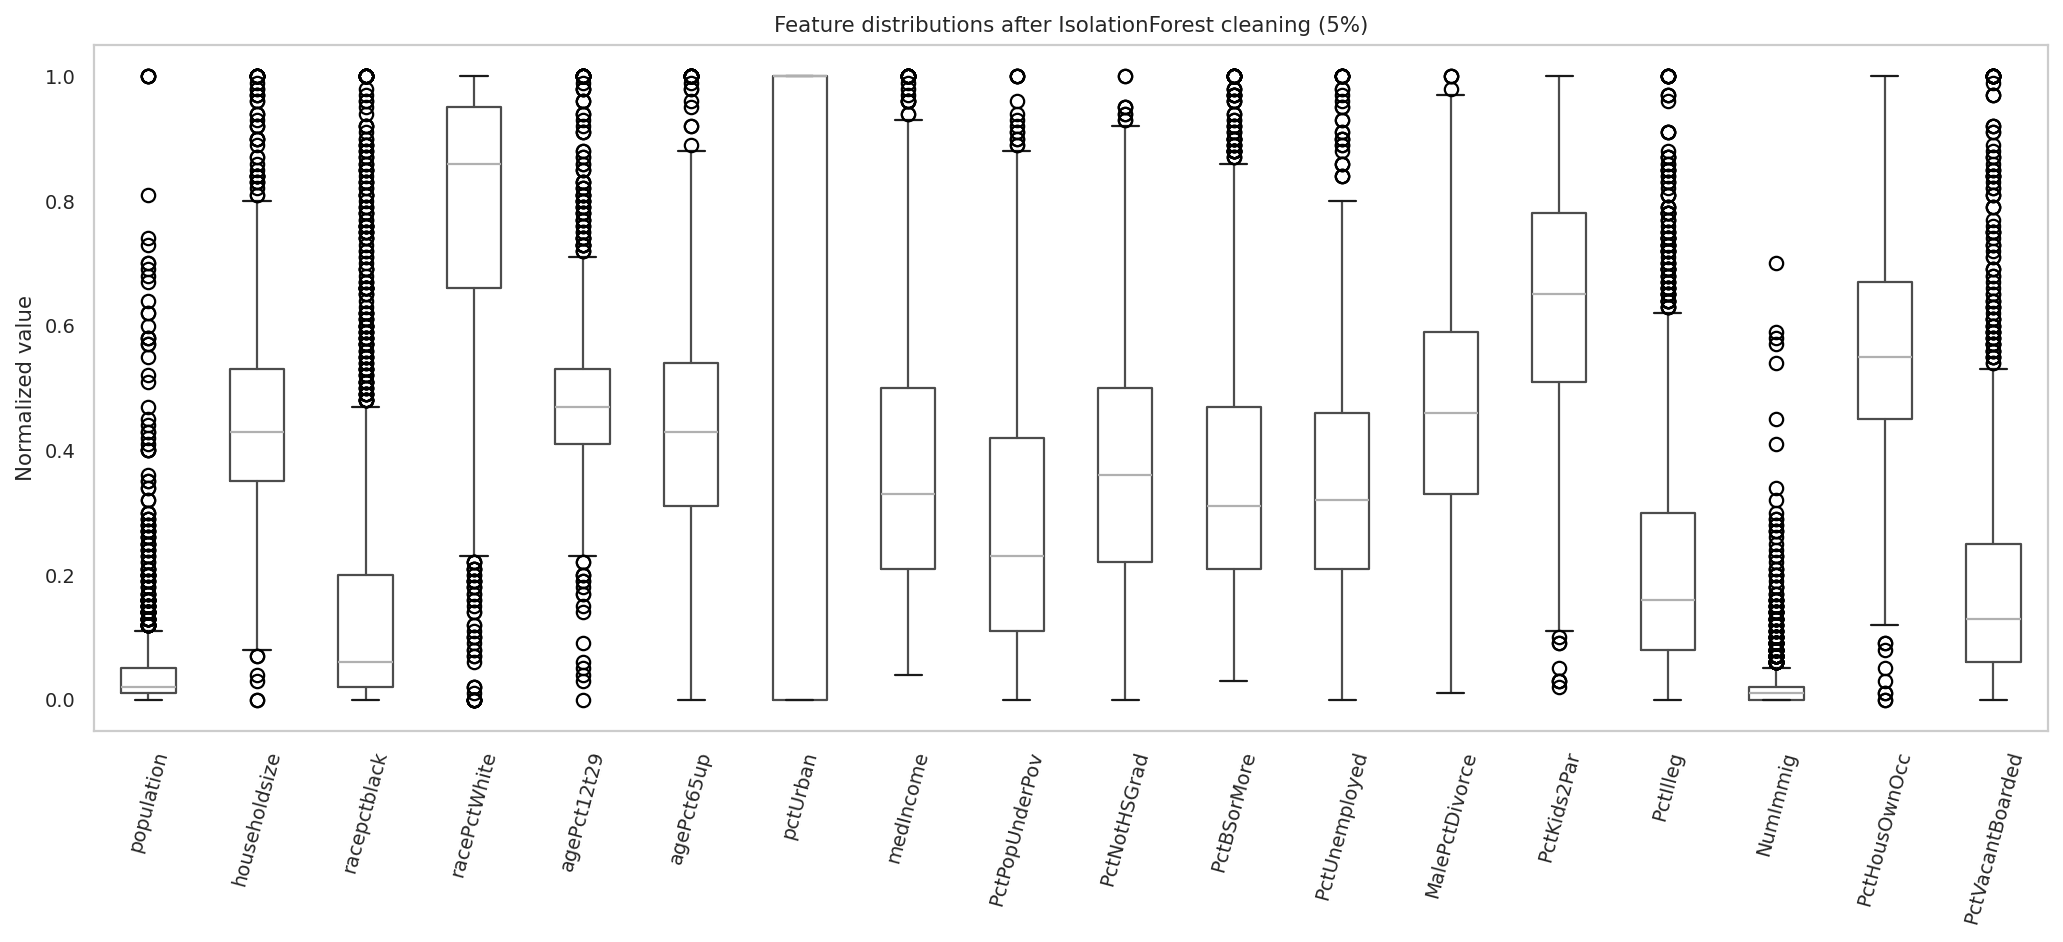
\includegraphics[width=\columnwidth]{boxplot_after.png}
\caption{Box plots after Isolation Forest cleaning (contamination $=0.05$). The most extreme tails of \texttt{population}, \texttt{NumImmig}, \texttt{PctIlleg}, and \texttt{PctVacantBoarded} are trimmed while the bulk of each distribution is preserved.}
\label{fig:box_after}
\end{figure}

The trimmed High-class shrinkage ($653\rightarrow 577$, $-11.6\%$) is now far milder than under per-feature IQR, while the qualitative shape of every feature distribution is preserved (Figure~\ref{fig:box_after}). All subsequent analyses use the cleaned dataset.

% ===================================================================
\section{Correlation Analysis (Task 2)}
\label{sec:corr}
The full Pearson correlation matrix among the eighteen features and the ordinally encoded class label is shown in Figure~\ref{fig:corrheat}. Several intuitive sociodemographic block structures emerge. Income, education, family stability, and home ownership form a positively correlated block (\texttt{medIncome}, \texttt{PctBSorMore}, \texttt{PctKids2Par}, \texttt{PctHousOwnOcc}), while indicators of deprivation form a separate positively correlated block (\texttt{PctPopUnderPov}, \texttt{PctNotHSGrad}, \texttt{PctUnemployed}, \texttt{PctVacantBoarded}, \texttt{PctIlleg}, \texttt{MalePctDivorce}). The two blocks are strongly anti-correlated with each other, reflecting the well-known socioeconomic gradient.

\begin{figure}[!t]
\centering
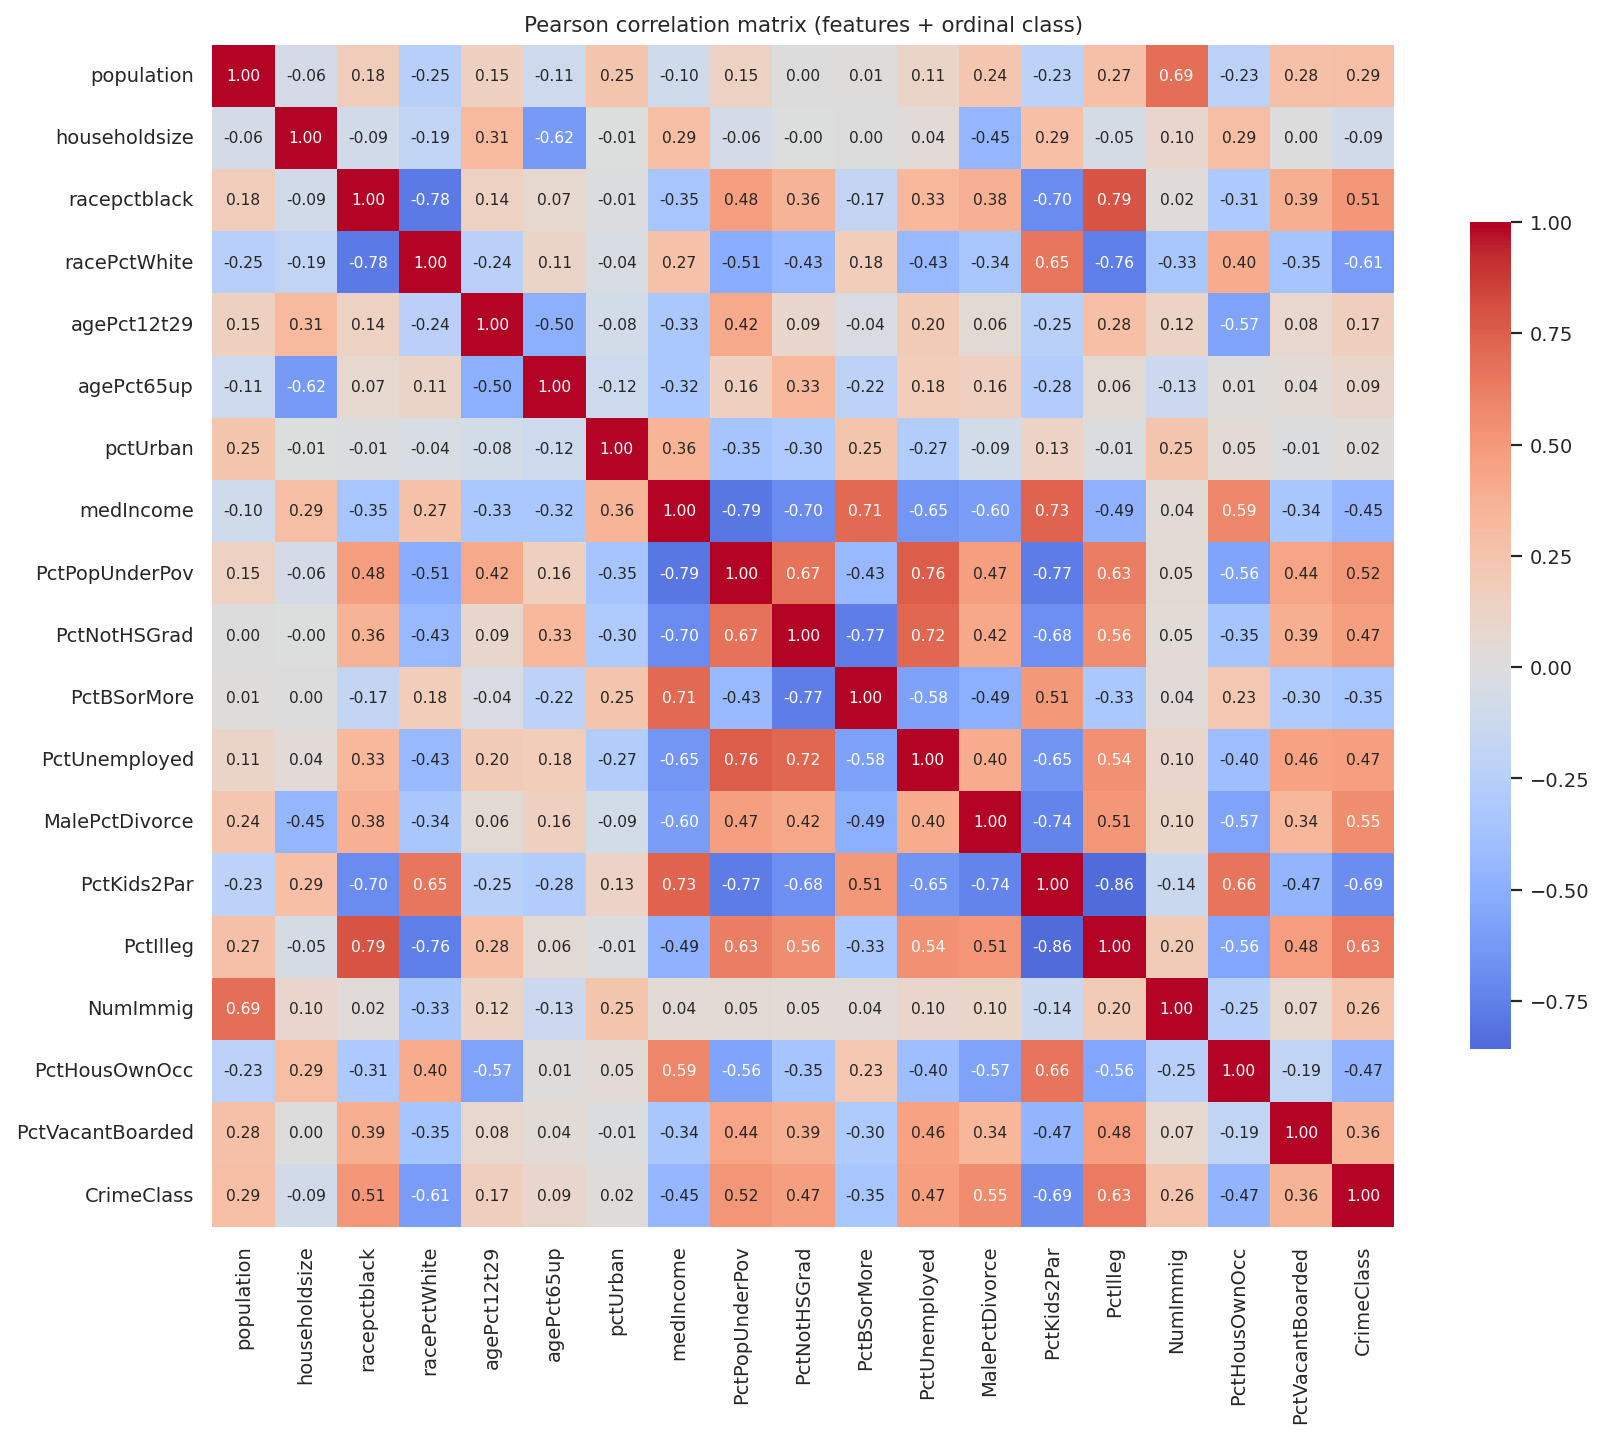
\includegraphics[width=\columnwidth]{correlation_heatmap.png}
\caption{Pearson correlation matrix of the eighteen features and the ordinally coded crime class.}
\label{fig:corrheat}
\end{figure}

\begin{figure}[!t]
\centering
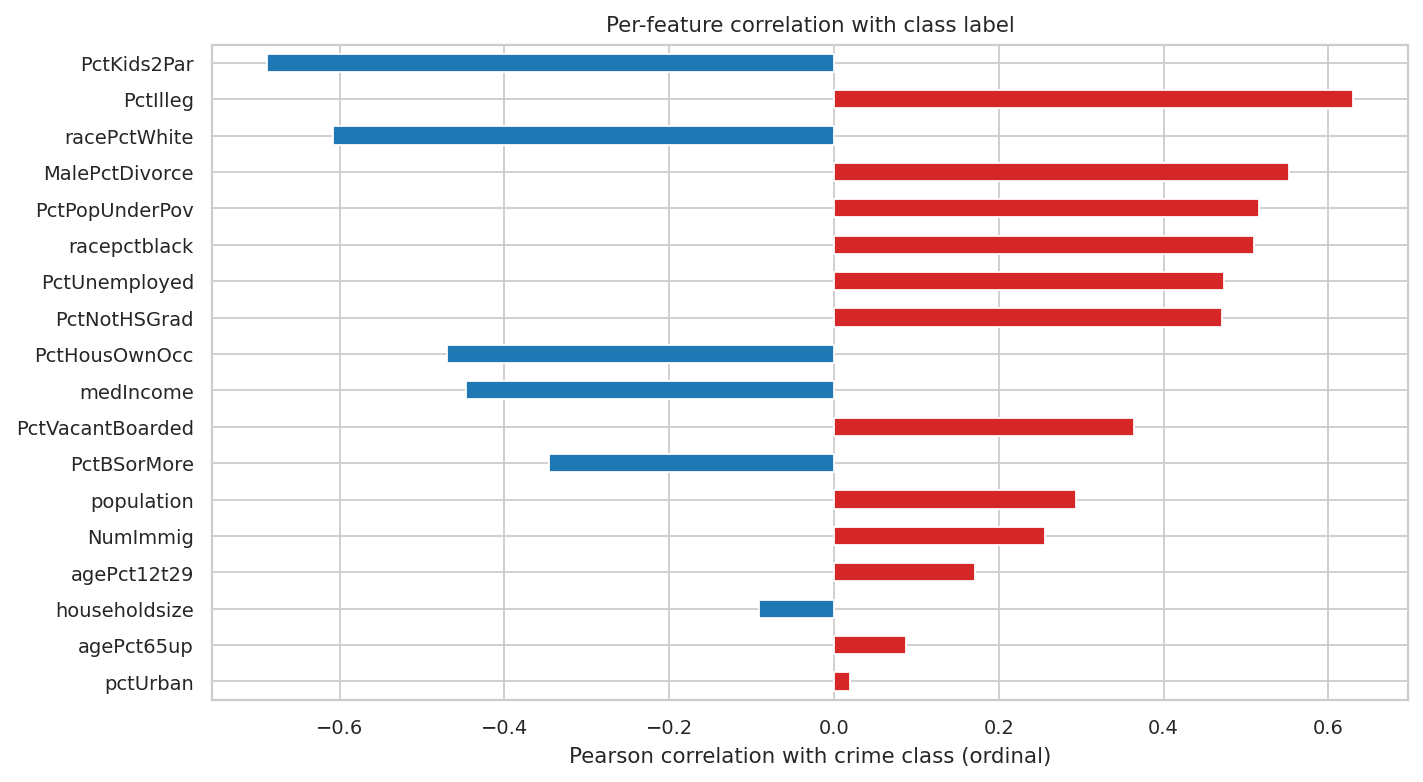
\includegraphics[width=\columnwidth]{feature_class_correlation.png}
\caption{Per-feature Pearson correlation with the (ordinal) crime class. Red bars indicate positive correlation with higher crime levels.}
\label{fig:classcorr}
\end{figure}

Figure~\ref{fig:classcorr} ranks features by absolute Pearson correlation with the (ordinal) crime class. The strongest individual correlates are \texttt{PctKids2Par} ($-0.69$), \texttt{PctIlleg} ($+0.63$), \texttt{racePctWhite} ($-0.61$), \texttt{MalePctDivorce} ($+0.55$), \texttt{PctPopUnderPov} ($+0.52$), and \texttt{medIncome} ($-0.45$). The signs are consistent with the established sociological literature on community-level crime: family stability, education, income, and home ownership are protective, while poverty, family disruption, unemployment, and housing decay co-occur with higher violent crime. Demographic-only variables such as \texttt{pctUrban}, \texttt{householdsize}, \texttt{agePct12t29}, and \texttt{agePct65up} carry very little individual class signal.

Because the class label is an \emph{ordinal} tertile rather than an interval-scale variable, the Spearman rank correlation was also computed for the feature-class relationship. The Spearman values are typically slightly stronger in magnitude (e.g., \texttt{PctKids2Par} $-0.70$, \texttt{PctIlleg} $+0.68$, \texttt{racePctWhite} $-0.64$), and the absolute-correlation \emph{ranking} of features under the two metrics is essentially identical (Spearman rank agreement $0.99$ between Pearson and Spearman rankings). This confirms that the qualitative conclusions of this section are not artefacts of treating the ordinal class label as interval-scaled.

% ===================================================================
\section{Z-Score Normalization and Per-Feature Fisher Distance (Task 3)}
\label{sec:fisher}
After z-scoring, the per-feature Fisher Distance was computed as a multi-class generalisation of the classical two-class Fisher score:
\begin{equation}
J(f) \;=\; \frac{\sum_{c=1}^{C} n_c\,(\mu_c^{(f)}-\mu^{(f)})^2}{\sum_{c=1}^{C}\sum_{i\in c}(x_i^{(f)}-\mu_c^{(f)})^2},
\label{eq:fisher}
\end{equation}
where $\mu_c^{(f)}$ is the class-$c$ mean of feature $f$ and $\mu^{(f)}$ is its global mean. Larger $J(f)$ indicates that feature $f$ separates the class means well relative to within-class dispersion.

\begin{figure}[!t]
\centering
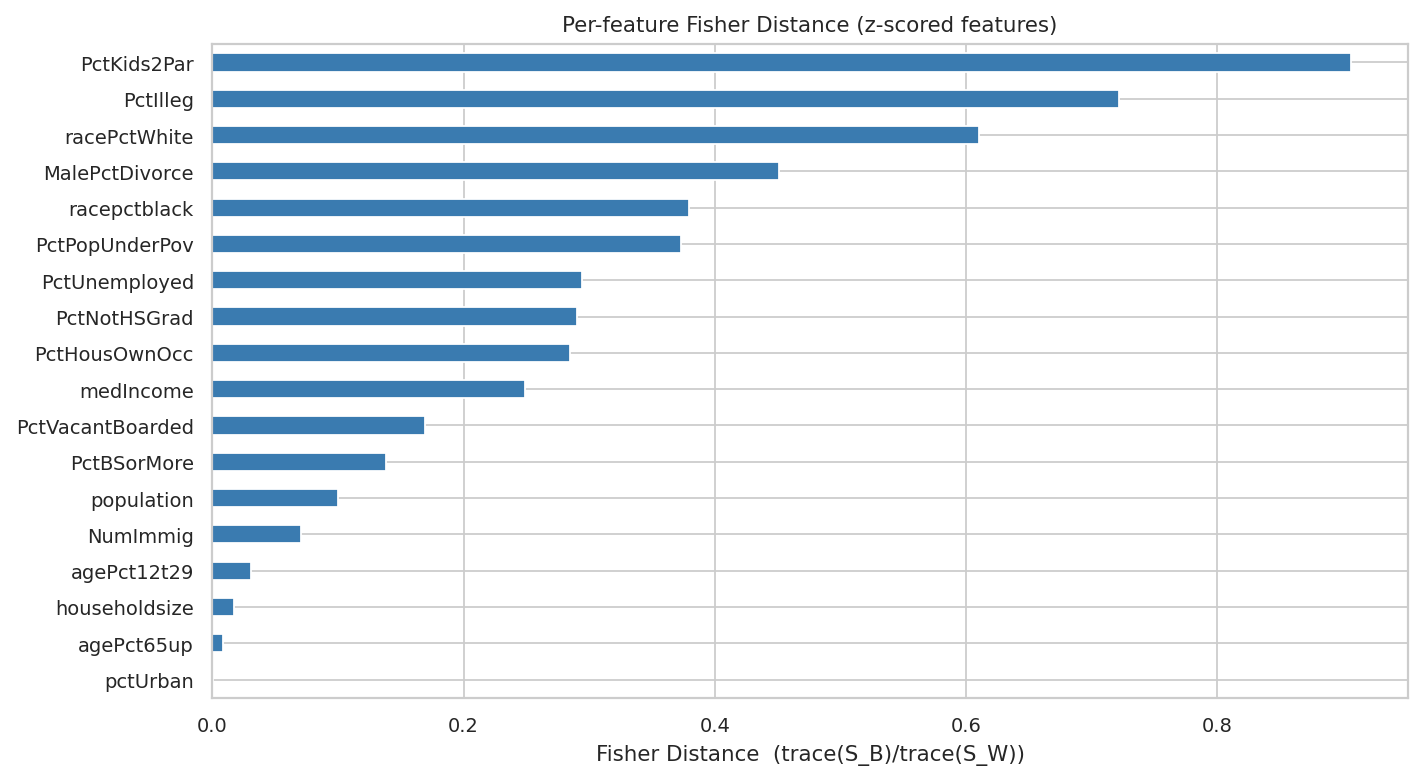
\includegraphics[width=\columnwidth]{fisher_features.png}
\caption{Per-feature Fisher Distance after z-score normalization. \texttt{PctKids2Par} and \texttt{PctIlleg} dominate.}
\label{fig:fisher_feat}
\end{figure}

The resulting ranking (Figure~\ref{fig:fisher_feat}) is largely consistent with the correlation ranking of Section~\ref{sec:corr}. The two top-ranked features are \texttt{PctKids2Par} ($J\!=\!0.91$) and \texttt{PctIlleg} ($J\!=\!0.72$), followed by \texttt{racePctWhite} ($0.61$), \texttt{MalePctDivorce} ($0.45$), and \texttt{racepctblack} ($0.38$). Features such as \texttt{pctUrban}, \texttt{householdsize}, and \texttt{agePct65up} have Fisher Distance values close to zero, indicating that their class-conditional distributions are nearly indistinguishable. The Fisher Distance and absolute class correlation rankings agree well, since for univariate normalized features both quantities effectively measure the contrast between class means relative to within-class scatter.

% ===================================================================
\section{PCA and Fisher Distance per Principal Component (Task 4)}
\label{sec:pca}
PCA was applied to the z-scored data, producing $18$ principal components. The leading component PC1 alone explains $39.2\%$ of the variance, and the first five components together account for $78.9\%$ of the total variance (Figure~\ref{fig:scree}). This is consistent with the strong correlation block-structure observed in Section~\ref{sec:corr}: a single socioeconomic ``advantage--disadvantage'' axis dominates the feature space.

\begin{figure}[!t]
\centering
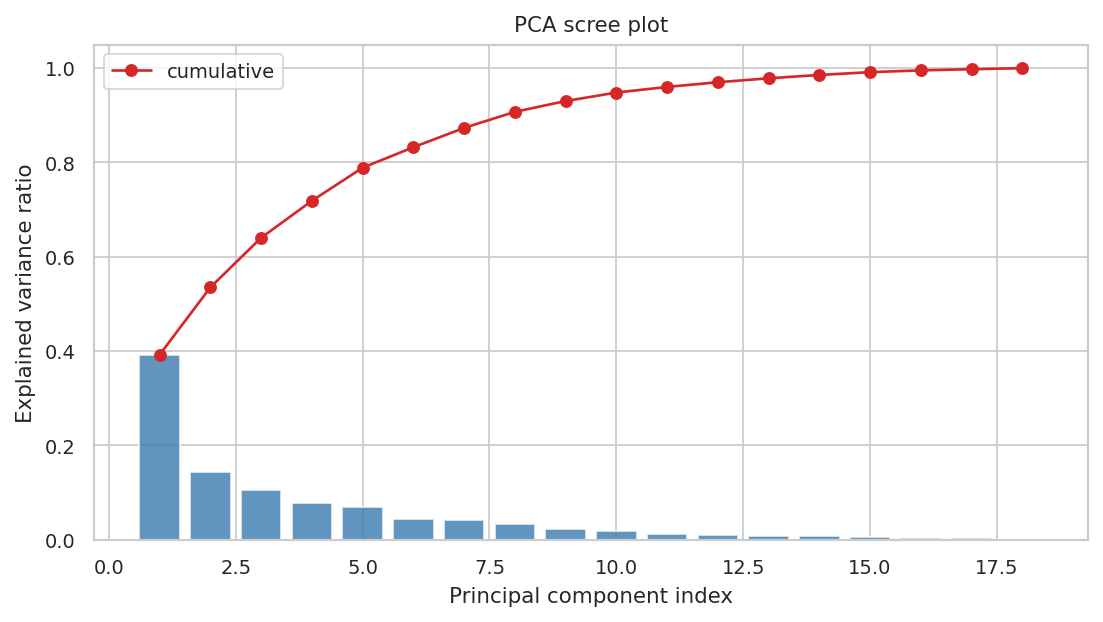
\includegraphics[width=\columnwidth]{pca_scree.png}
\caption{PCA scree plot. PC1 captures $39.2\%$ of the variance; the top five components capture $78.9\%$.}
\label{fig:scree}
\end{figure}

Treating each PC projection as a feature, the Fisher Distance from Equation~(\ref{eq:fisher}) was recomputed (Figure~\ref{fig:fishercmp}). The Fisher Distance of PC1 is $0.86$, which is the second-highest score in the entire study (only the original \texttt{PctKids2Par} feature, with $J=0.91$, scores higher). All other principal components have Fisher Distance below $0.04$.

\begin{figure}[!t]
\centering
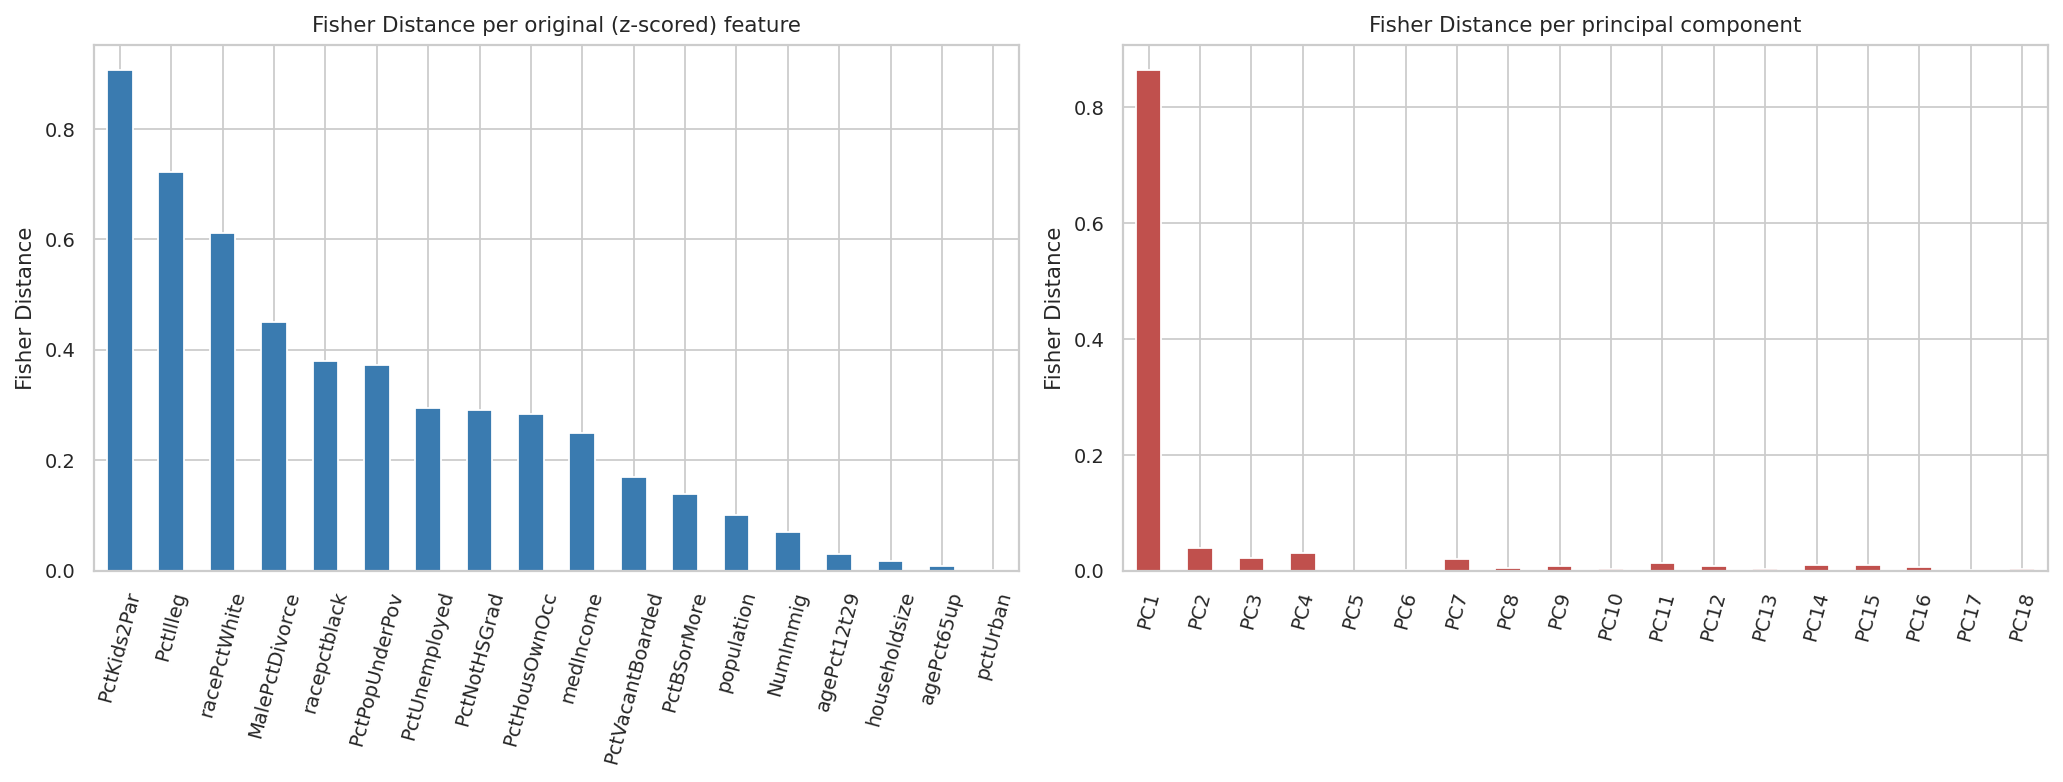
\includegraphics[width=\columnwidth]{fisher_comparison.png}
\caption{Per-feature Fisher Distance for the z-scored original features (left) and for the $18$ principal components (right). PC1 inherits most of the discriminative content of the leading correlated block of features.}
\label{fig:fishercmp}
\end{figure}

\begin{figure}[!t]
\centering
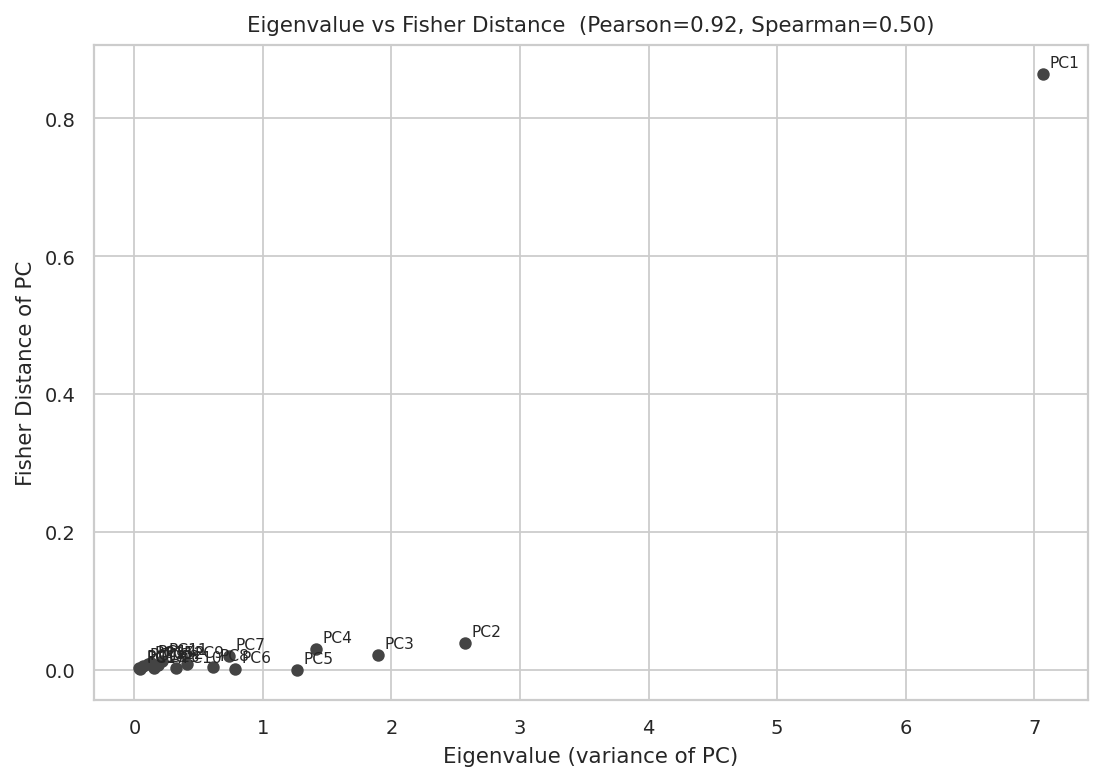
\includegraphics[width=0.95\columnwidth]{eigval_vs_fisher.png}
\caption{Eigenvalue versus Fisher Distance for the $18$ principal components. Pearson correlation $r=0.92$, Spearman $\rho=0.50$.}
\label{fig:eigfisher}
\end{figure}

There is a strong positive relationship between the eigenvalue of a principal component (its variance) and its Fisher Distance: the Pearson correlation between the two is $r=0.92$ and the Spearman rank correlation is $\rho=0.50$ (Figure~\ref{fig:eigfisher}). The result, however, must be interpreted with care. The high Pearson coefficient is driven almost entirely by PC1, which is a strong outlier with both the largest eigenvalue and by far the largest Fisher Distance. The rank correlation $\rho=0.50$ is more informative: among the remaining PCs, higher-variance components tend to be more class-discriminative, but the ordering is far from strict (several mid-variance components such as PC11 and PC4 in fact carry slightly more class signal than the lower-variance PC5--PC10). This is consistent with the theoretical observation that PCA maximizes variance, not class separability; the alignment between the leading PCA direction and the discriminative direction here is a property of this particular dataset, where the dominant axis of variation \emph{is} the socioeconomic gradient that drives the crime class.

% ===================================================================
\section{Scatter Plots on the First and Last Two PCs (Task 5)}
\label{sec:pcscatter}
Figure~\ref{fig:pcscat} shows the projection of the cleaned data onto the two most important and the two least important principal components, with samples coloured by their true class label.

\begin{figure}[!t]
\centering
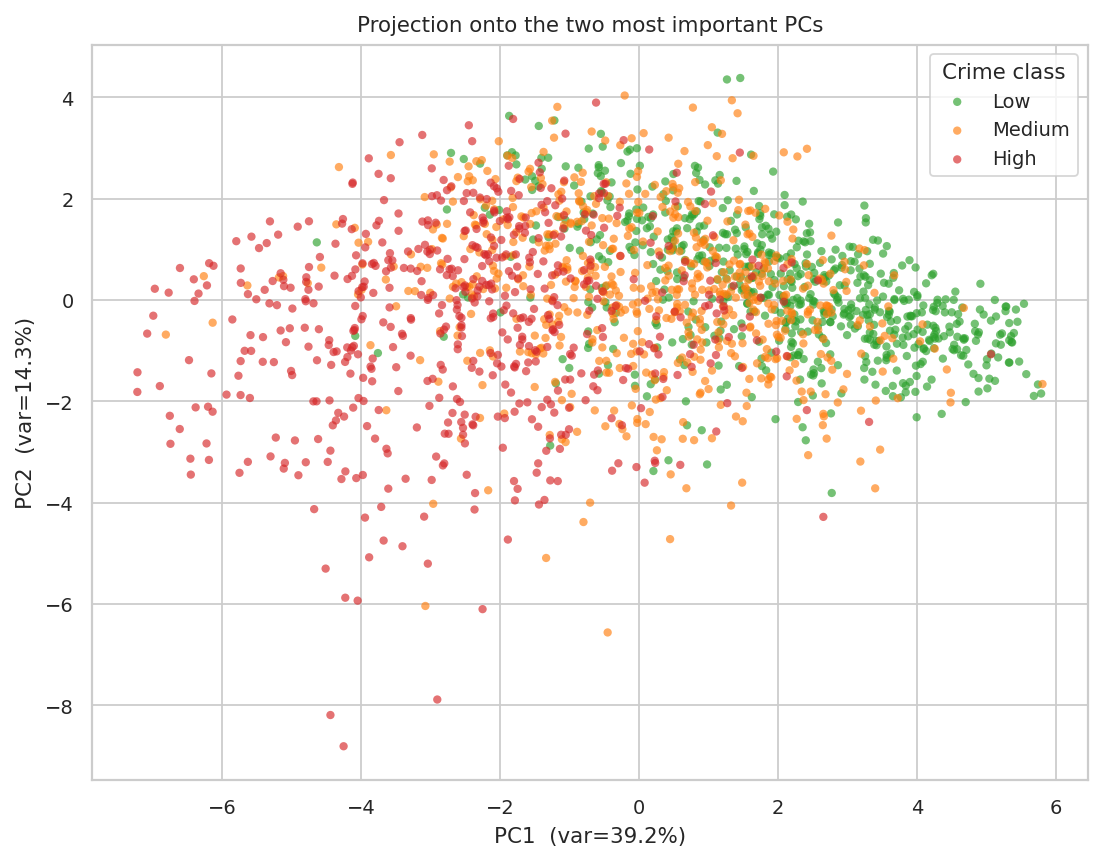
\includegraphics[width=\columnwidth]{pca_top2.png}
\\[2pt]
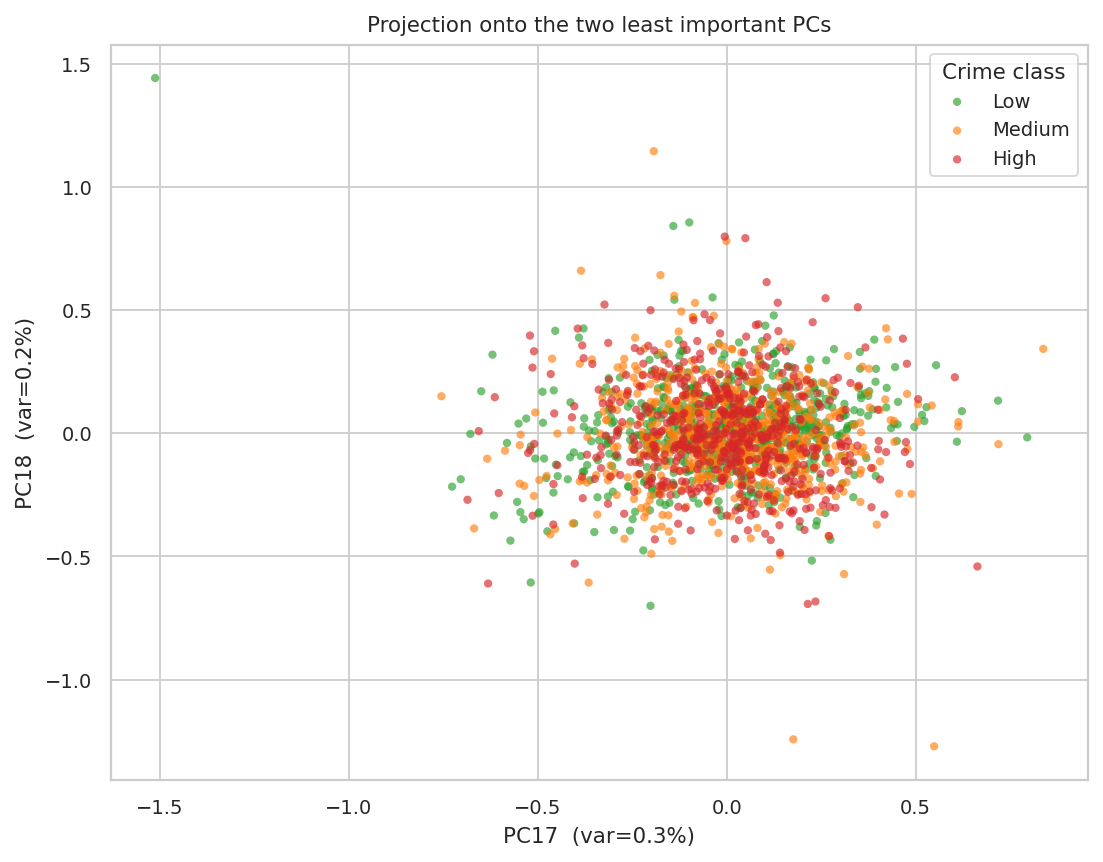
\includegraphics[width=\columnwidth]{pca_bottom2.png}
\caption{Top: projection onto (PC1, PC2). A clear monotone ordering Low $\rightarrow$ Medium $\rightarrow$ High emerges along PC1. Bottom: projection onto the two least important PCs, which show no class structure.}
\label{fig:pcscat}
\end{figure}

The (PC1, PC2) plot shows a clean, almost monotone gradient: \emph{Low}-crime communities concentrate on the negative side of PC1, \emph{High}-crime communities on the positive side, and \emph{Medium} communities form an overlapping band in between. PC2 contributes little additional separation. In contrast, the projection onto the two least important PCs shows essentially no class structure: the three classes are interleaved in a small isotropic cloud, which is expected because these components capture noise-like residual variance.

% ===================================================================
\section{LDA Projection and Class-Separability Comparison (Task 6)}
\label{sec:lda}
A Linear Discriminant Analysis was fit with $n_{\text{components}}=2$. By construction, LDA maximizes between-class scatter relative to within-class scatter and therefore tends to produce a tighter class-separable 2-D embedding than PCA when class information is available.

\begin{figure}[!t]
\centering
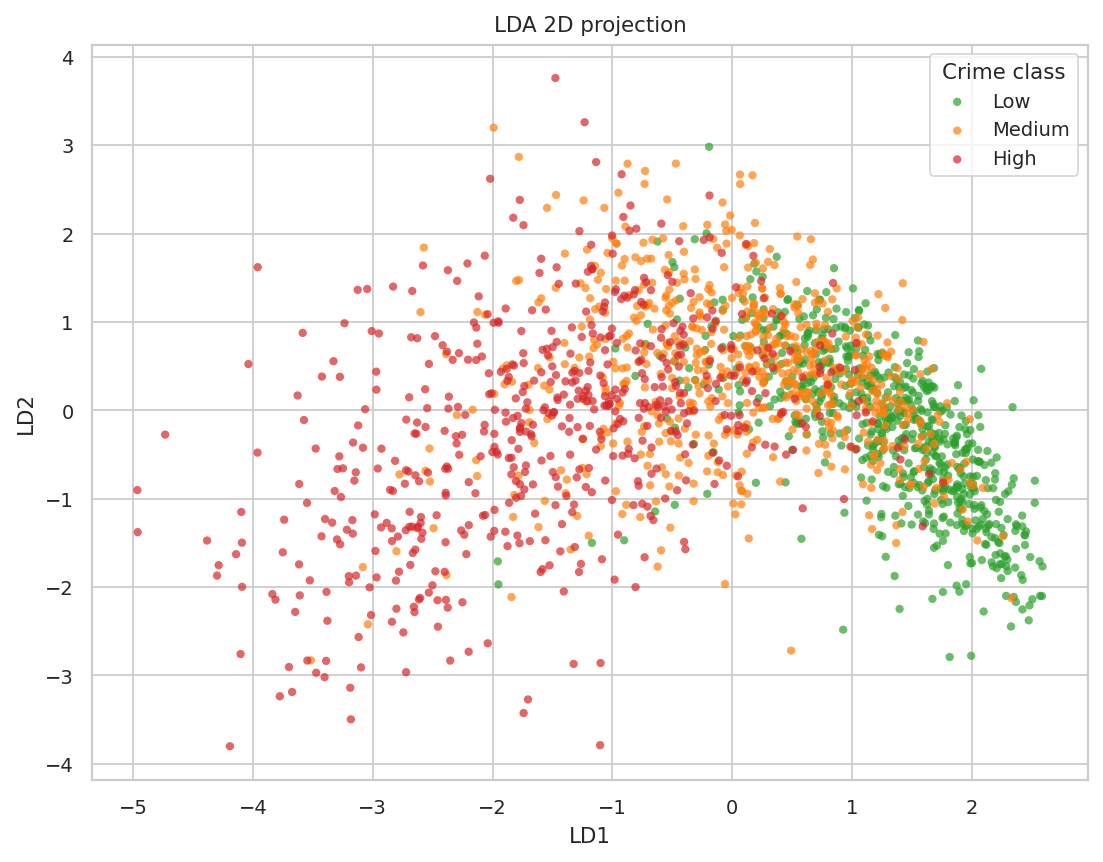
\includegraphics[width=\columnwidth]{lda_scatter.png}
\caption{LDA 2-D projection. The three classes form a clearer left--right ordering than in the PCA projection.}
\label{fig:lda}
\end{figure}

\begin{table}[!t]
\caption{Quantitative separability of the 2-D PCA and LDA embeddings. Higher is better in both cases.}
\label{tab:sep}
\centering
\begin{tabular}{lcc}
\toprule
Metric & PCA (PC1,PC2) & LDA (LD1,LD2) \\
\midrule
Silhouette (true labels) & $0.070$ & $0.112$ \\
5-NN accuracy (5-fold CV) & $0.583$ & $0.638$ \\
\bottomrule
\end{tabular}
\end{table}

To make the comparison quantitative, two metrics were computed on the 2-D embeddings (Table~\ref{tab:sep}). The silhouette coefficient (with the true class labels as the partition) increases by $60\%$ from PCA ($0.070$) to LDA ($0.112$). The mean 5-fold cross-validated accuracy of a 5-NN classifier trained on the 2-D embedding also improves from $58.3\%$ on PCA to $63.8\%$ on LDA, a relative gain of $+5.5$ percentage points. Both metrics confirm visually what Figures~\ref{fig:pcscat} and \ref{fig:lda} suggest: LDA reveals tighter class separability than PCA. The improvement is bounded because, as Section~\ref{sec:pca} showed, the leading PCA direction is already strongly aligned with the discriminative direction; LDA's advantage lies in additionally exploiting class labels to deflate the within-class scatter along the second discriminant axis.

% ===================================================================
\section{Clustering Comparison: K-Means, DBSCAN, t-SNE, SOM (Task 7)}
\label{sec:cluster}
The four algorithms were applied with two different inputs as required by the assignment. K-Means ($k\!=\!3$) and DBSCAN ($\varepsilon\!=\!0.5$, $\mathrm{minPts}\!=\!10$) operate on the 2-D PCA projection (PC1, PC2). t-SNE (perplexity $30$, PCA initialization) and a $12\times 12$ MiniSom \cite{minisom} are fit on the full $18$-dimensional z-scored data.

\begin{figure}[!t]
\centering
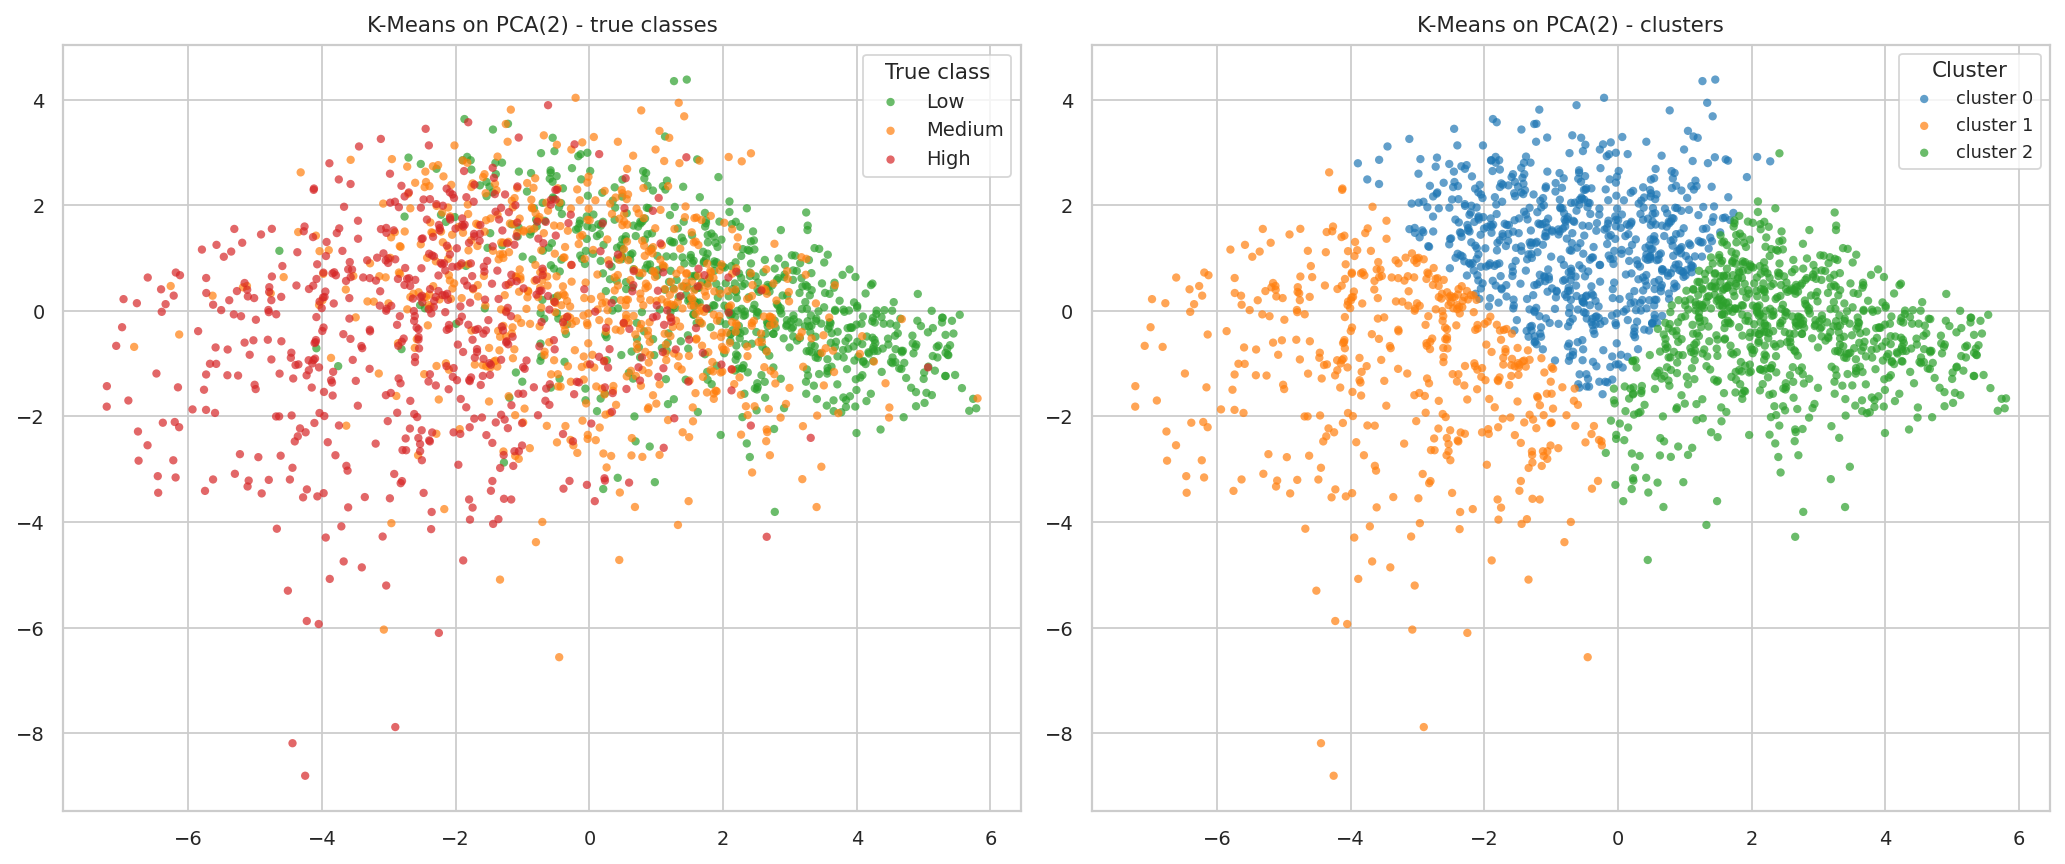
\includegraphics[width=\columnwidth]{cluster_kmeans.png}
\caption{K-Means ($k=3$) on the (PC1, PC2) projection. Left: true classes; right: assigned clusters.}
\label{fig:kmeans}
\end{figure}

\begin{figure}[!t]
\centering
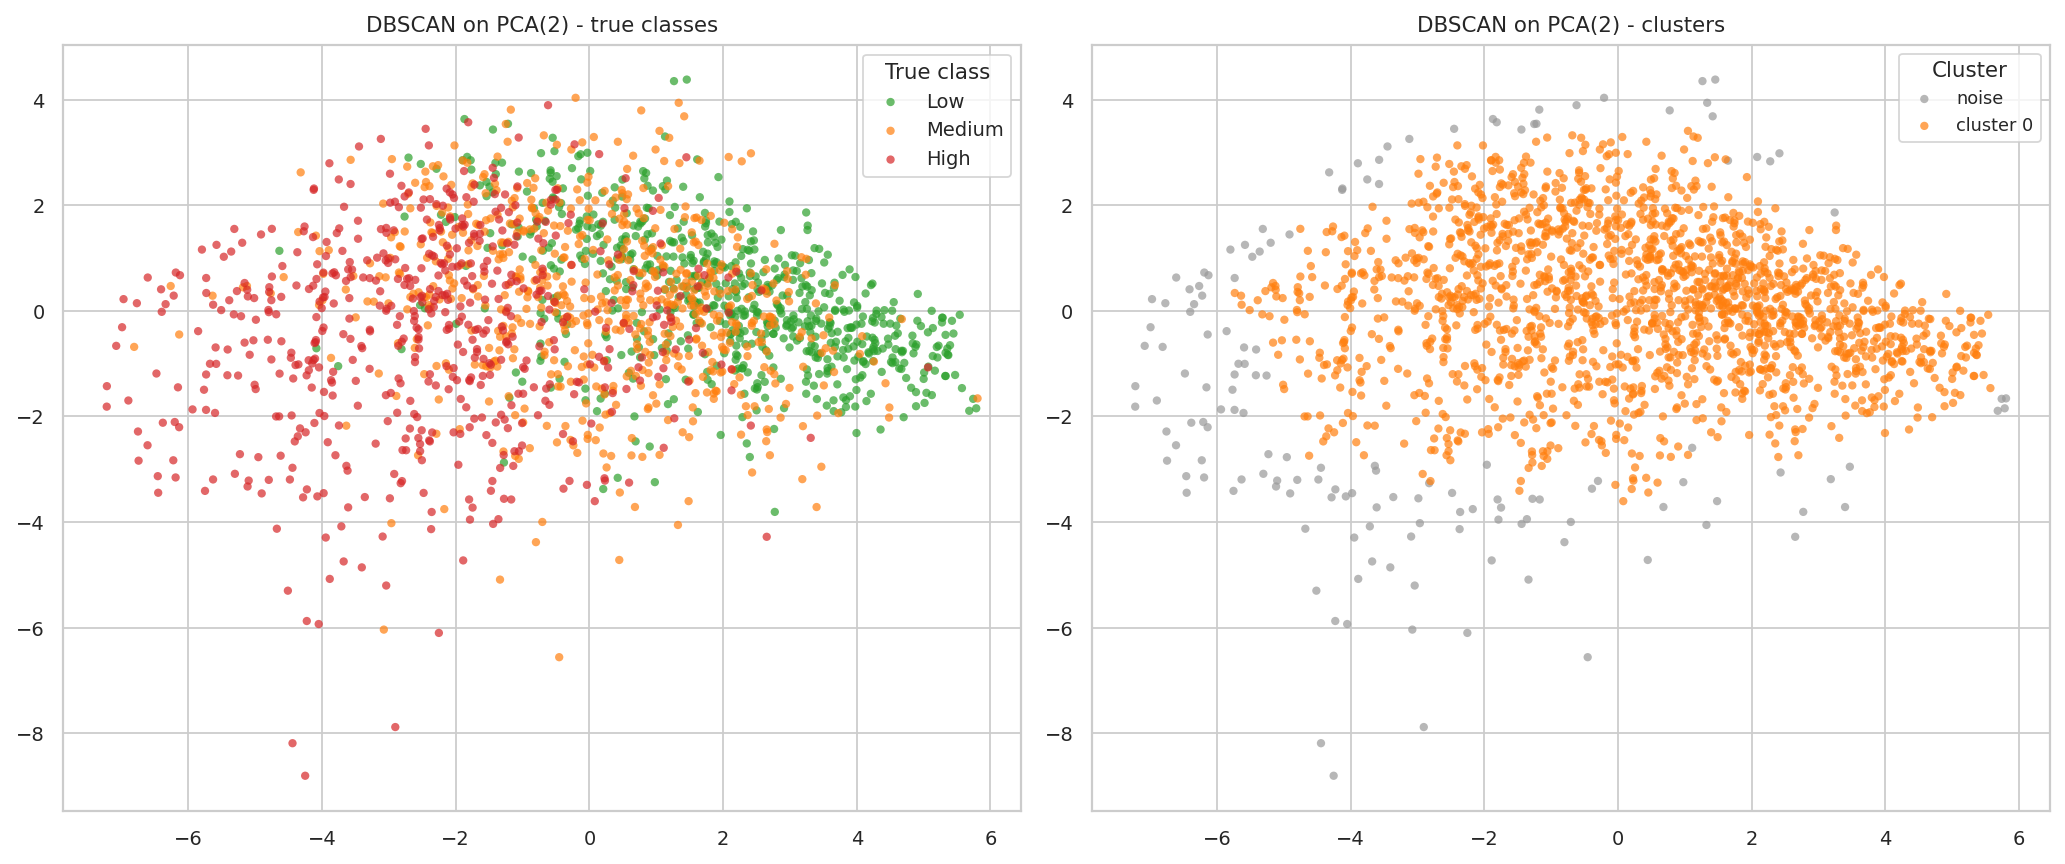
\includegraphics[width=\columnwidth]{cluster_dbscan.png}
\caption{DBSCAN ($\varepsilon=0.5$, $\mathrm{minPts}=10$) on (PC1, PC2). The bulk of the data collapses into a single dense cluster with $150$ samples ($7.9\%$) flagged as noise.}
\label{fig:dbscan}
\end{figure}

\begin{figure}[!t]
\centering
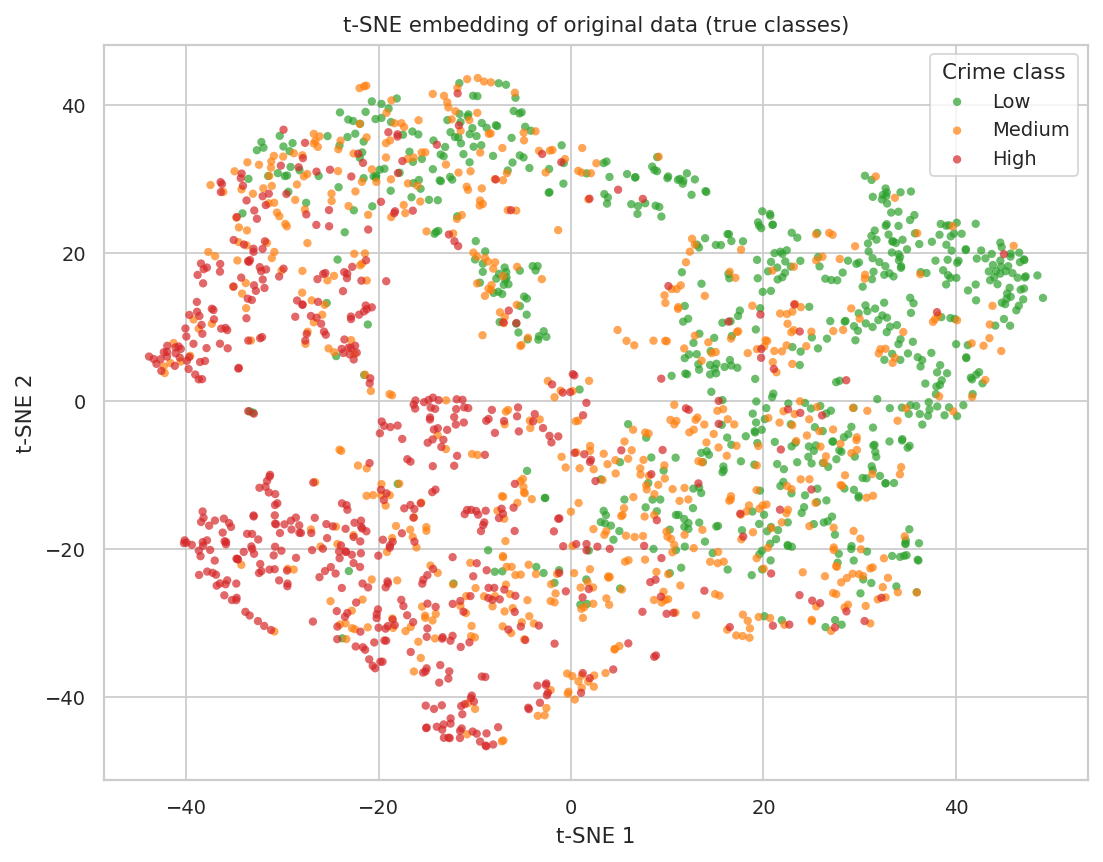
\includegraphics[width=\columnwidth]{cluster_tsne.png}
\caption{t-SNE embedding of the full $18$-dimensional z-scored data, coloured by true class. A continuous gradient is visible across the embedding.}
\label{fig:tsne}
\end{figure}

\begin{figure}[!t]
\centering
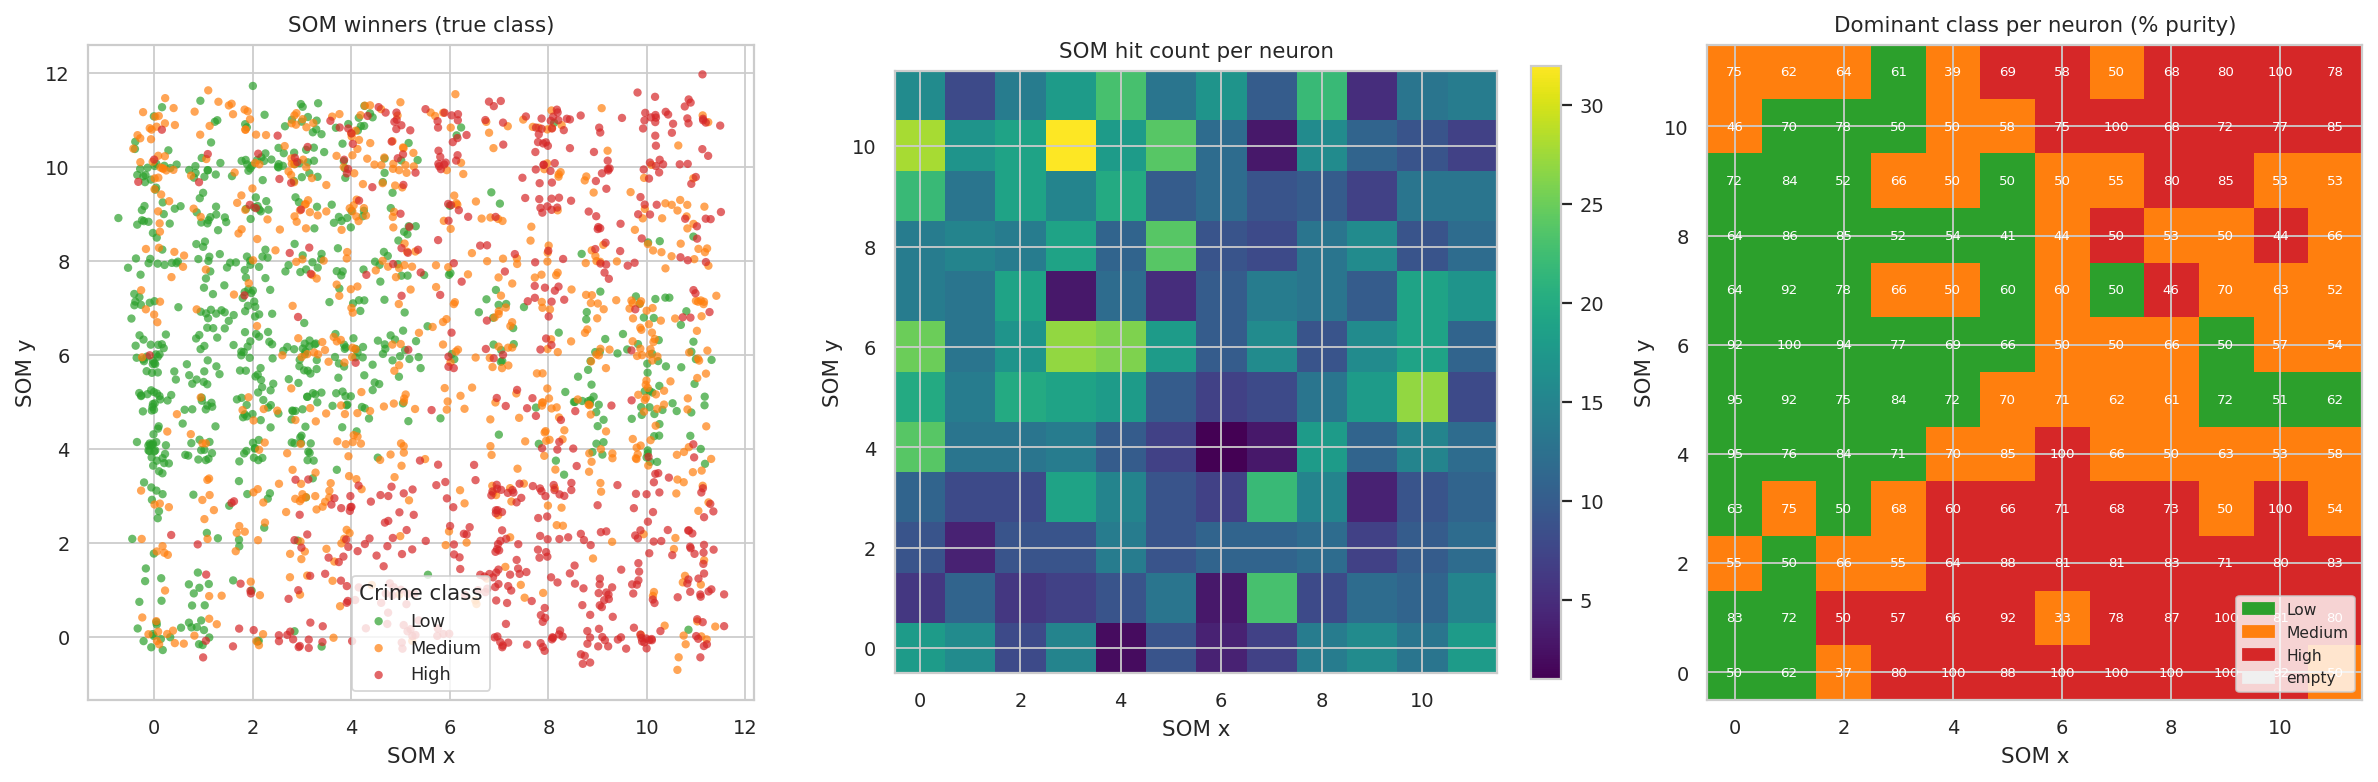
\includegraphics[width=\columnwidth]{cluster_som.png}
\caption{$12\times 12$ MiniSom trained on the original z-scored data. Left: scatter of winners coloured by true class (jittered for visibility). Centre: per-neuron hit-count heat-map. Right: dominant class per neuron with per-cell purity (text labels, in $\%$); the mean purity of non-empty cells is $69\%$.}
\label{fig:som}
\end{figure}

\begin{table}[!t]
\caption{Adjusted Rand Index (ARI) and Normalised Mutual Information (NMI) between cluster assignments and the true class labels.}
\label{tab:clust}
\centering
\begin{tabular}{lcc}
\toprule
Method (input) & ARI & NMI \\
\midrule
K-Means, $k=3$ (PCA-2D)  & $0.202$ & $0.215$ \\
DBSCAN ($\varepsilon=0.5$) (PCA-2D) & $0.019$ & $0.050$ \\
\bottomrule
\end{tabular}
\end{table}

\paragraph{K-Means} on the (PC1, PC2) plane recovers three clusters whose boundaries are essentially vertical cuts along PC1. This is consistent with the structure seen in Section~\ref{sec:pcscatter}: PC1 carries almost all of the class signal, so unsupervised partitioning along PC1 already gives non-trivial agreement with the true labels (ARI $=0.20$, NMI $=0.22$). However, the agreement is far from perfect because the three classes overlap heavily along PC2.

\paragraph{DBSCAN} essentially fails: at $\varepsilon=0.5$, $\mathrm{minPts}=10$ it finds a single dense cluster plus $150$ noise points (ARI $=0.02$). Because the data form a single continuous ``socioeconomic gradient'' rather than well-separated density modes, density-based clustering cannot recover the three classes; DBSCAN exposes that the class structure of this dataset is gradient-like, not modal.

\paragraph{t-SNE} on the full $18$-dimensional data produces a single, smoothly curved manifold along which the three classes form a continuous gradient (\emph{Low} on one side, \emph{High} on the other). This visualisation reinforces the picture that the classes are largely defined by position along a one-dimensional socioeconomic continuum, not by separate compact clusters.

\paragraph{SOM} The $12\times 12$ MiniSom grid (Figure~\ref{fig:som}) provides the most class-organised non-linear view. The hit-count heat-map (centre panel) shows that the SOM allocates capacity smoothly across the grid with two slightly heavier hubs. The dominant-class panel (right) reveals contiguous regions of Low, Medium, and High classes arranged along an approximately diagonal gradient on the lattice, with several cells reaching $\geq 90\%$ purity. The mean per-neuron purity over non-empty cells is $69\%$, well above the $\approx 35\%$ expected from chance under the (near-uniform) class distribution. The SOM thus confirms, on the original feature space, the same gradient-like organisation seen in the t-SNE map.

% ===================================================================
\section{Hypothesis Test on \texttt{PctKids2Par} (Task 8)}
\label{sec:hypothesis}
The feature \texttt{PctKids2Par} (percentage of kids living in two-parent households) was selected for the hypothesis test because it has the largest Fisher Distance and the largest absolute correlation with the class label (Sections~\ref{sec:corr}--\ref{sec:fisher}). The hypothesis to be tested is the equality of its mean between the \emph{Low} and \emph{High} crime classes:
\begin{align*}
H_0:\ \mu_{\text{Low}} = \mu_{\text{High}}, \qquad
H_1:\ \mu_{\text{Low}} \neq \mu_{\text{High}}.
\end{align*}
Two independent random samples of sizes $n=36$ and $n=64$ were drawn (without replacement) from each class, and a two-sided Welch's t-test (which does not assume equal variances) was applied. The results are summarized in Table~\ref{tab:ttest}.

\begin{table}[!t]
\caption{Welch's t-test results on \texttt{PctKids2Par} between the Low and High crime classes.}
\label{tab:ttest}
\centering
\begin{tabular}{lccc}
\toprule
$n$ per class & $\bar x_{\text{Low}}$ ($\pm$ s.d.) & $\bar x_{\text{High}}$ ($\pm$ s.d.) & $t$ \ ($p$-value) \\
\midrule
$36$ & $0.786\pm 0.118$ & $0.471\pm 0.155$ & $9.65$ \ ($1.9\!\times\!10^{-14}$) \\
$64$ & $0.811\pm 0.099$ & $0.476\pm 0.165$ & $12.99$ \ ($1.9\!\times\!10^{-23}$) \\
all  & $-$              & $-$              & $39.89$ \ ($\approx 10^{-214}$) \\
\bottomrule
\end{tabular}
\end{table}

In all three settings (samples of size $36$, $64$, and the full classes) the p-value is many orders of magnitude smaller than any conventional significance level $\alpha\in\{0.05, 0.01, 0.001\}$. The null hypothesis of equal means is therefore rejected with overwhelming evidence in favour of $H_1$: \texttt{PctKids2Par} is, on average, substantially higher in Low-crime communities than in High-crime communities (approximately $0.80$ vs.\ $0.47$ on the normalized scale, a $\approx 0.33$ shift on a $[0,1]$ scale). As expected, increasing the sample size from $36$ to $64$ leaves the sample means almost unchanged but increases $|t|$ from $9.65$ to $12.99$, illustrating the higher statistical power of a larger sample for the same effect size. The full-class $t=39.89$ extrapolates this trend to the limit of the available data.

% ===================================================================
\section{Conclusion}
\label{sec:conclusion}
This project applied a complete exploratory and statistical analysis pipeline to the UCI Communities and Crime dataset, with the continuous violent-crime rate discretized into three classes. The following coherent picture emerges. First, family-structure and socioeconomic variables (\texttt{PctKids2Par}, \texttt{PctIlleg}, \texttt{PctPopUnderPov}, \texttt{MalePctDivorce}, \texttt{racePctWhite}, \texttt{medIncome}) carry the strongest individual class signal, as confirmed independently by both Pearson and Spearman correlation and by per-feature Fisher Distance (Spearman--Pearson rank agreement $0.99$), while purely demographic variables such as \texttt{pctUrban}, \texttt{householdsize}, \texttt{agePct12t29}, and \texttt{agePct65up} are essentially class-uninformative. Second, the discriminative content is concentrated along a single principal direction: PC1 alone explains $39.2\%$ of the variance and obtains a Fisher Distance ($0.86$) higher than every original feature except \texttt{PctKids2Par}. Eigenvalues and Fisher Distances of principal components are strongly positively correlated in raw value ($r=0.92$) but only moderately so in rank ($\rho=0.50$): high variance does not strictly imply high discriminability beyond the dominant component. Third, the LDA 2-D embedding outperforms the PCA 2-D embedding in revealing class separability, both visually and quantitatively (silhouette $0.112$ vs.\ $0.070$; 5-NN CV accuracy $63.8\%$ vs.\ $58.3\%$). Fourth, unsupervised clustering reveals that the class structure of this dataset is gradient-like rather than modal: K-Means partitions PC1 into three slabs and recovers moderate agreement with the labels (ARI $0.20$), DBSCAN collapses to a single dense cluster with $150$ noise points, and both t-SNE and SOM produce a continuous manifold along which the three classes shade smoothly into each other; nevertheless the SOM achieves a mean per-neuron class purity of $69\%$, well above the chance level. Finally, a Welch's t-test on \texttt{PctKids2Par} rejects the null hypothesis of equal class means with extreme significance at both $n=36$ ($t=9.65$) and $n=64$ ($t=12.99$), formally confirming the descriptive evidence of the earlier sections.

Overall, the dataset is best understood not as three well-separated clusters but as a one-dimensional socioeconomic continuum along which violent crime rises monotonically. This explains why simple linear methods (PCA, LDA) capture most of the available structure, why density-based clustering fails, and why the strongest individual predictors are family-structure and deprivation indicators rather than purely demographic ones.

\appendix
\section{A}
The Jupyter notebook implementing the full analysis pipeline (\texttt{Crime\_Analysis.ipynb}) and all generated figures accompany this report. The original dataset is publicly available from the UCI Machine Learning Repository \cite{uciccrime}.

\begin{thebibliography}{1}
\bibitem{uciccrime}
M.~Redmond, ``Communities and Crime Data Set,'' UCI Machine Learning Repository, 2009. [Online]. Available: \url{https://archive.ics.uci.edu/ml/datasets/communities+and+crime}
\bibitem{minisom}
G.~Vettigli, ``MiniSom: minimalistic and NumPy-based implementation of the Self Organizing Map,'' 2018. [Online]. Available: \url{https://github.com/JustGlowing/minisom}
\bibitem{pedregosa}
F.~Pedregosa \emph{et al.}, ``Scikit-learn: Machine Learning in Python,'' \emph{Journal of Machine Learning Research}, vol.~12, pp.~2825--2830, 2011.
\bibitem{liu2008isolation}
F.~T.~Liu, K.~M.~Ting, and Z.-H.~Zhou, ``Isolation Forest,'' in \emph{Proc.\ 2008 Eighth IEEE Int.\ Conf.\ on Data Mining (ICDM)}, 2008, pp.~413--422.
\end{thebibliography}

\begin{IEEEbiography}[{
\includegraphics[width=1in,height=1.25in,clip,keepaspectratio]{serkan_vek.jpg}}]{Serkan Eren}
received his B.Sc.\ degree in Electronics Engineering from Gebze Technical University, T\"urkiye, in 2023, and is currently pursuing an M.Sc.\ degree in Artificial Intelligence at the same institution. He works as an Automotive Software Engineer at FEV T\"urkiye, contributing to Python-based automation, DevOps pipelines, and embedded software integration. His professional interests include deep learning, software engineering for intelligent systems, and the development of data-driven applications for automation and natural language processing.
\end{IEEEbiography}

\EOD
\end{document}
